\section{Präliminarien}
\subsection{Komplexe Zahlen}
Wenn man mit den reellen Zahlen arbeitet, bekommt man Probleme, wenn man die Wurzel aus einer negativen Zahl zieht. Jedoch haben Mathematiker im 17. Jahrhundert eine Lösung für dieses Problem entdeckt, indem dieses Zahlensystem mit den imaginären Zahlen, die die imaginäre Einheit i haben, erweitert wird (Geschichte des Zahlenbegriffs 1970, S.66). Addieren und Subtrahieren zweier imaginären Zahlen funktioniert genau gleich, wie wenn man mit einer reellen Zahl rechnet. Dies heisst, dass das i wie die 'herkömmlichen' Variablen behandelt werden kann. Jedoch muss man beim Multiplizieren, Dividieren und beim somit entstehenden Rechnen mit Potenzen aufpassen, denn es gilt für $n \in \mathbb{Z}$:
% Gleichunugen
\begin{align*}
\text{i}^{4n} &= 1 \\
\text{i}^{4n+1} &= \text{i} \\
\text{i}^{4n+2} &= -1 \\
\text{i}^{4n+3} &= -\text{i}
\end{align*}
%Weiter im Text
Man sollte Potenzen mit der Basis i nach den oben genannten Regeln vereinfachen. Hier sieht man gut, dass eine Verknüpfung zwischen den imaginären und reellen Zahlen in die andere Direktion ebenfalls existiert. Wenn man nun eine imaginäre Zahl $\text{i}b$ mit einer reellen Zahl $a$ zusammenaddiert, bekommt man eine komplexe Zahl  $c=a+\text{i}b$ mit dem Realteil $a$ und dem Imaginärteil $b$. $a$ und $b$ sind hier reelle Zahlen. Beim Addieren von komplexen Zahlen $z=a+\text{i}b$ und $w=e+\text{i}f$ folgt man diesem Beispiel:
\[z+w\]
\[a+\text{i}b+e+\text{i}f\]
\[a+e+(b+f)\text{i}\]
Nun merkt man, dass eine komplexe Zahl mit einem Vektor vergleichbar ist, denn um die Zahl darstellen zu können, benutzt man die 2-dimensionale komplexe Ebene (Mathematik - Die faszinierende Welt der Zahlen 2015, S. 144). Daraus schliesst sich, dass komplexe Zahlen 2-dimensional sind. Multipliziert man eine komplexe Zahl und beobachtet dies auf der komplexen Ebene, fängt der Punkt an, scheinbar unkontrolliert herumspringen. Der Punkt folgt jedoch weiterhin logischen Regeln. Beim Quadrieren verschiebt sich der Punkt in die positive Drehrichtung (Gegenuhrzeigersinn).
\\
Ebenfalls kann, da die Zahl vergleichbar mit einem Vektor ist, der absolute Betrag der komplexen Zahl $c$ bestimmt werden, welcher mit dem Pythagoras berechnet wird (Ein Weg zur fraktalen Geometrie 1989, S. 22):
\[|c| = |a+\text{i}b| = \sqrt[2]{a^2+b^2}\]

\subsection{Fraktale Geometrie}
\subsubsection{Allgemein}
Um zum Buddhabrot zu kommen, müssen wir noch einen weiteren Begriff klären: das Fraktal.\\ Würde bei einem 3$n$ grossem Strich der mittlere Drittel fehlen, an dieser die anderen zwei Seiten eines gleichseitigen Dreiecks mit der Seitenlänge $n$ stehen, hätte man die erste Iteration einer Kochkurve. Würde man nun in die einzelnen $n$ grosse Striche die vorige Iteration der Kochkurve einfügen, entsteht die zweite Iteration. Man kann dies ab nun immer wieder machen, sodass ein immer detaillierteres und komplizierteres Bild entsteht.\\

\begin{figure}[h]
    \centering
    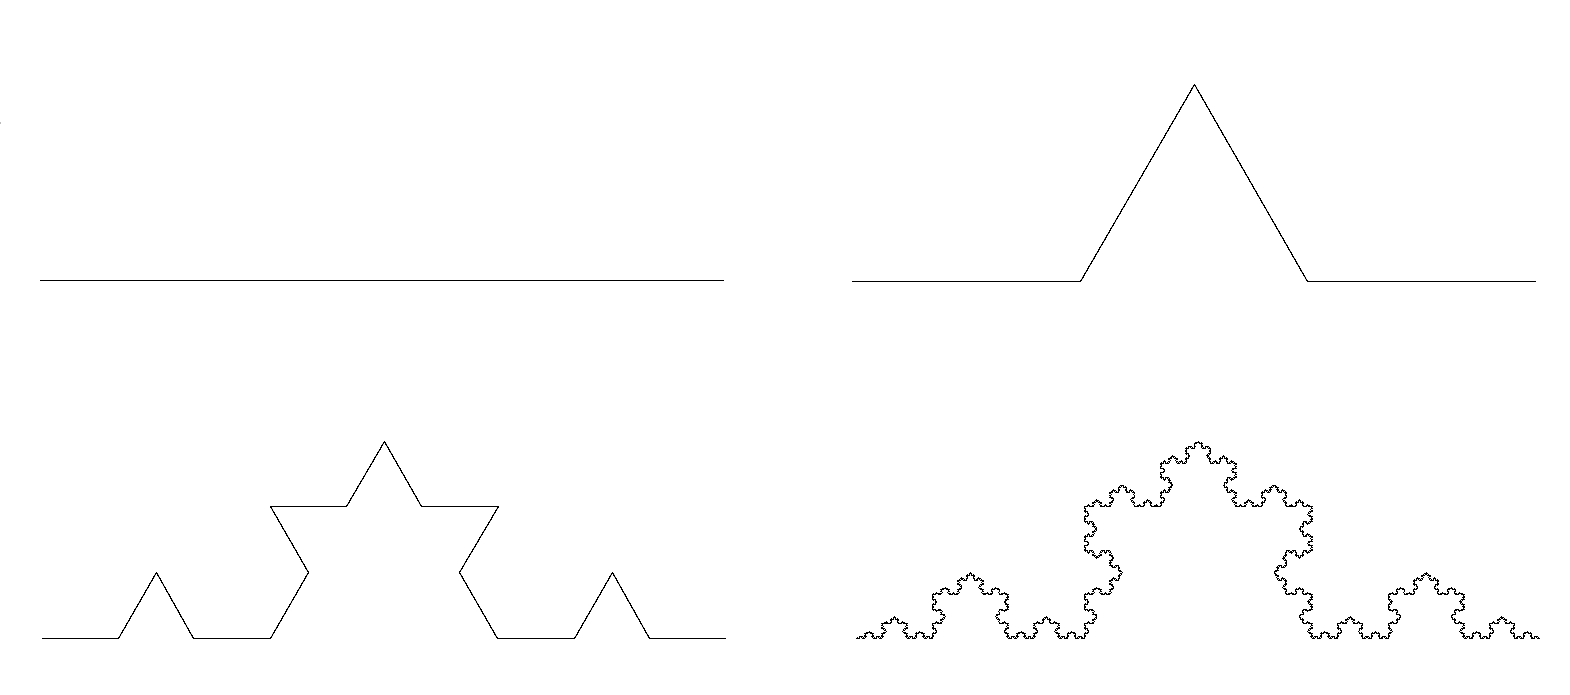
\includegraphics[width=.5\textwidth]{Pictures/Kochkurve.png}
    \caption{Die Entstehung der Kochkurve}
    \label{fig:Kochkurve}
\end{figure}
Wenn man in die Kochkurve hineinzoomt, findet man die Kochkurve immer wieder: ein rekursives Bild oder eben ein Fraktal (Lexikon der Mathemathik - 3 2001, S. 128).\\Man definiert nun das Fraktal als eine Figur, bei der sehr oft Selbstähnlichkeit auffindbar ist, das heisst, dass das gesamte Fraktal oder Teile davon mehrfach im Fraktal vorkommen und das Fraktal selbst eine gebrochene und somit keine ganzzahlige Dimension besitzt (Mathematik - Die faszinierende Welt der Zahlen 2015, S. 258).\\

\subsubsection{Mandelbrotmenge}
Die nach dem Mathematiker Benoît B. Mandelbrot (*20.11.1924; †14.10.2010) benannte Menge ($\mathbb{M}$) beinhaltet jede Zahl $c$ die nicht gegen $\infty$ divergiert für folgende Folge (Ein Weg zur fraktalen Geometrie 1989, S. 54):
\begin{align*}
z_0&=0\\
z_{n+1}&=z^2_n+c
\end{align*}
Man fand heraus, dass wenn $|z_n| > 2$ gilt, wird die Folge gegen $\infty$ divergieren (Ein Weg zur fraktalen Geometrie 1989, S. 74).\\
Die erstellte Abbildung, je nachdem mit ein bisschen Farbe dazu, ergibt ein sehr schönes Gebilde, welches die deutschsprachigen Leute aufgrund seiner Form an ein 'Apfelmännchen' erinnerte, weshalb es von ihnen auch so genannt wird (Ein Weg zur fraktalen Geometrie 1989, S. 54).\\
Die $\mathbb{M}$ ist ein Fraktal (Mathematik - Die faszinierende Welt der Zahlen 2015, S. 258). Man findet das erst gesehene Bild der Menge beim Hineinzoomen immer wieder, somit ist es ebenfalls selbstähnlich. Immer wieder findet man verschiedene Julia-Mengen mit dem Zugehörigem $c$ (Ein Weg zur fraktalen Geometrie 1989, S. 54). Diese sind ebenfalls Fraktale und sehen dazu auch noch für die Norm der Menschheit schön aus. $\mathbb{M}$ besitzt durch die vorgegebene Formel ein chaotisches System (Ein Weg zur fraktalen Geometrie 1989, S. 32).\\
All dies führt sicher dazu, dass es einige YouTube-Videos gibt, die einen Zoom in die Menge zeigen, welche auch viel Rechenleistung brauchen.

\subsubsection{Buddhabrot}
Schaut man den Namen als Erstes an, merkt man, dass das Wort 'Buddha' vom meditierenden Buddha kommt, denn dieser ist in der Abbildung ersichtlich. Ebenfalls fällt das Wort 'Brot' auf. Dies ist eine Andeutung, dass diese Abbildung etwas mit dem Mandelbrot zu tun hat, denn es stellt eine andere Variante dar, die $\mathbb{M}$ abzubilden.\\ 
Das Bild entsteht, indem das Mandelbrot nochmals berechnet wird, jedoch nur die Punkte, die bei der Mandelbrotberechnung gegen das $\infty$ divergieren. Nun wird auch nicht mehr geschaut, nach wie vielen Schritten der Punkt $c$ ins $\infty$ abdriftet, sondern bei welchen Punkten $c$ nach jeder Iteration landet.\\
Ebenfalls wird ein Zoom in das Buddhabrot durch das chaotische System von $\mathbb{M}$ und durch die fraktalen und selbstähnlichen Eigenschaften von $\mathbb{M}$ interessant.